\documentclass[10pt]{beamer}

\usetheme[progressbar=frametitle]{metropolis}
\usepackage{appendixnumberbeamer}
\usepackage{multicol}
\usepackage{booktabs}
\usepackage[scale=2]{ccicons}
\usepackage[style=authoryear]{biblatex}
\bibliography{demo.bib}
\usepackage{pgfplots}
\usepackage{bbm}
\usepackage{import}
\usepackage{graphics}


\usepgfplotslibrary{dateplot}


\usepackage{xspace}
\newcommand{\themename}{\textbf{\textsc{metropolis}}\xspace}

\title{Labor Markets and Technological Change: Evidence from Electronic Health Records}

\subtitle{Hanna Glenn}
 \date{\today}
% \date{}
%\author{Presented by: Hanna Glenn}
% \institute{Center for modern beamer themes}
% \titlegraphic{\hfill\includegraphics[height=1.5cm]{logo.pdf}}

\begin{document}

\maketitle

\setbeamercolor{background canvas}{bg=white}

\begin{frame}{Table of Contents}
  \setbeamertemplate{section in toc}[sections numbered]
  \tableofcontents%[hideallsubsections]
\end{frame}

\section[Motivation]{Motivation}

\begin{frame}{What is an EHR?}
\begin{itemize}
    \item Technology purchased and implemented by hospitals
\end{itemize}

\begin{itemize}
    \item Used for:
    \vspace{3mm}
    \begin{itemize}
        \item Electronic patient records
        \vspace{3mm}
        \item More complex (and expensive) EHRs allow for decision making assistance
        \vspace{3mm}
        \item Continuing to evolve over time
    \end{itemize}
\end{itemize}
\end{frame}

\begin{frame}[fragile]{HIT: Great (Expected) Potential in Healthcare}
\begin{alertblock}{Cost Saving}
\begin{itemize}
    \item Possible cost reduction of hundreds of billions of dollars \\ (\cite{hillestad2005})
\end{itemize}
\end{alertblock}

\begin{alertblock}{Quality Improvement}
\begin{itemize}
    \item Improved efficiency, patient safety improvements, physicians have decision support that could prevent unnecessary complications, etc.
    \item Significant policy push for EHR implementation: HITECH Act, 2008 provided financial incentive for hospitals to implement EHRs \nocite{hitech}
\end{itemize}
\end{alertblock}

\textcolor{blue}{The percentage of hospitals with basic EHR capability rose from 9$\%$ in 2008 to 84$\%$ in 2015.} (\cite{stats})

\end{frame}

\begin{frame}[fragile]{What does this mean for physicians?}
Immediate Effects:
\begin{itemize}
    \item Large startup costs (time, productivity)
    \item Possible loss of autonomy
\end{itemize}

Long Run Effects:
\begin{itemize}
    \item Productivity could increase or decrease
    \item Progressing loss of autonomy as technology progresses
\end{itemize}

\end{frame}

\begin{frame}[noframenumbering]{Physician Burnout in the Media}
\begin{center}
    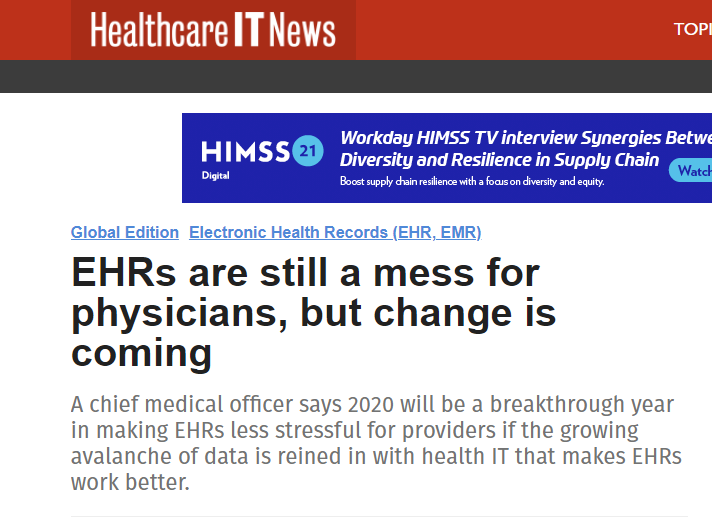
\includegraphics[scale=.4]{graphics/News Clip1.PNG}
\end{center}
\end{frame}

\begin{frame}[noframenumbering]{Physician Burnout in the Media}
\begin{center}
    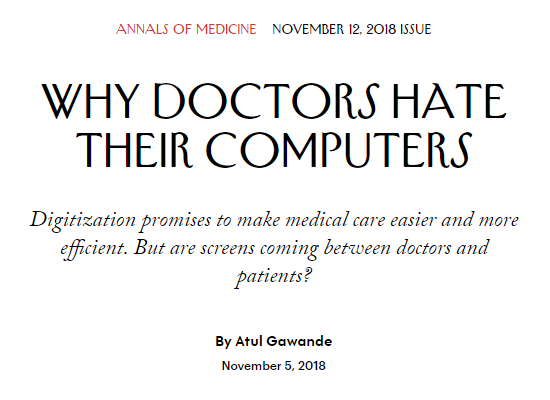
\includegraphics[scale=.5]{graphics/News Clip2.PNG}
\end{center}
\end{frame}

\begin{frame}[noframenumbering]{Physician Burnout in the Media}
\begin{center}
    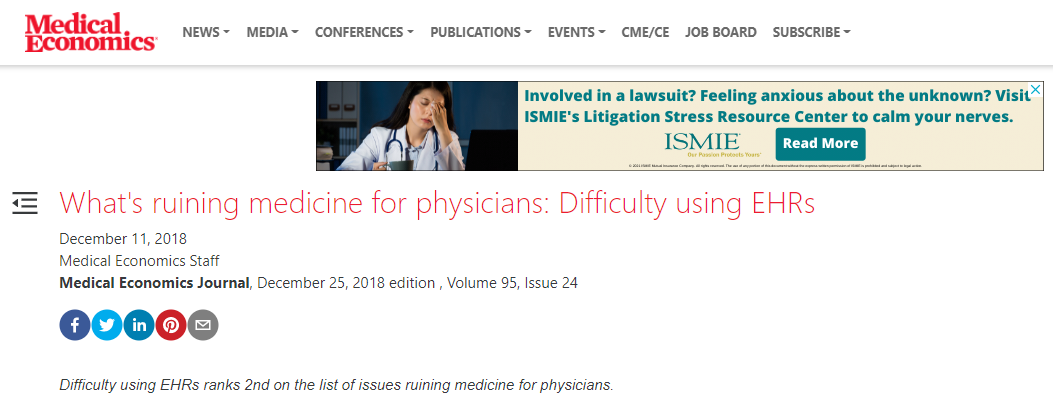
\includegraphics[scale=.45]{graphics/News Clip3.PNG}
\end{center}
\end{frame}

\begin{frame}{This Paper}

Did EHR implementation in hospitals affect physician labor outcomes?
\begin{itemize}
    \item Intensive Margin / Productivity
    \item Extensive Margin
    \item Hospital $\rightarrow$ Office?
\end{itemize}
\end{frame}


\section{Contribution}

\begin{frame}{Literature}
    
\end{frame}





\section{Data}


\begin{frame}{What I Want to Capture}
\begin{itemize}
    \item Initial Implementation
    \begin{itemize}
        \item Productivity gains/losses
        \item Immediate changes to labor market decisions: retirement or place of work
    \end{itemize}
    \item Loss of autonomy and cost of learning/using new technology
    \begin{itemize}
        \item Could cause physicians to move to settings where they have more control
    \end{itemize}
\end{itemize}


\end{frame}

\begin{frame}{About the Data}
    Main measurements come from \underline{CMS Shared Patient Data} (2009-2015)
    \begin{itemize}
        \item Lists 2 NPIs and the number of billings those two entities shared in the same day
    \end{itemize}
    
    How I use it:
    \begin{itemize}
        \item Limit the NPIs to physician-hospital pairs, where physicians are PCPs, internists, hospitalists
        \item Limit the billings to those which occur in the same day
        \item Only keep pairs with sufficient number of billings together to suggest a close relationship between physician and hospital
        \item Aggregate to the physician level to avoid spillover effects
    \end{itemize}
\end{frame}


\begin{frame}{Measures of Physician Labor Market Decisions}


     Total hospital patients: 
    \begin{itemize}
        \item Sum of shared patients with all hospitals
    \end{itemize}
     
     \vspace{4mm}
     
     Indicator for switching work setting:
    \begin{itemize}
        \item Positive billings shared with all entities but shared entities with hospitals becomes 0
        \item \color{gray}{SK$\&$A database of office-based physicians}
    \end{itemize}
    
    \vspace{4mm}
    
    \textcolor{gray}
     {Indicator for retirement/ leaving the labor force}

\end{frame}

\begin{frame}{Measure of EHR Use}

Physician-level treatment variable that captures exposure to \textit{any} EHR
\begin{itemize}
    \item Individual hospital EHR use comes from AHA survey
    \item Treatment turns on the first time any of the shared hospitals implements an EHR
\end{itemize}
\end{frame}


\begin{frame}{Other Characteristics}

Medical school graduation date, gender: \underline{Physician Compare}

\vspace{5mm}

Average size of hospital worked with (measured in beds), average hospital days operating: \underline{AHA Survey}
\end{frame}

\begin{frame}{Summary Statistics}
\centering
    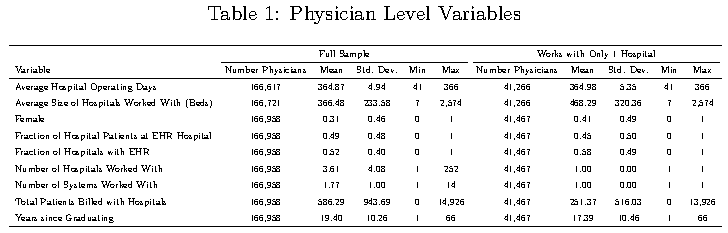
\includegraphics[scale=.8]{Objects/sumstats.pdf}
\end{frame}

\begin{frame}{Physician EHR Use}
    \centering
    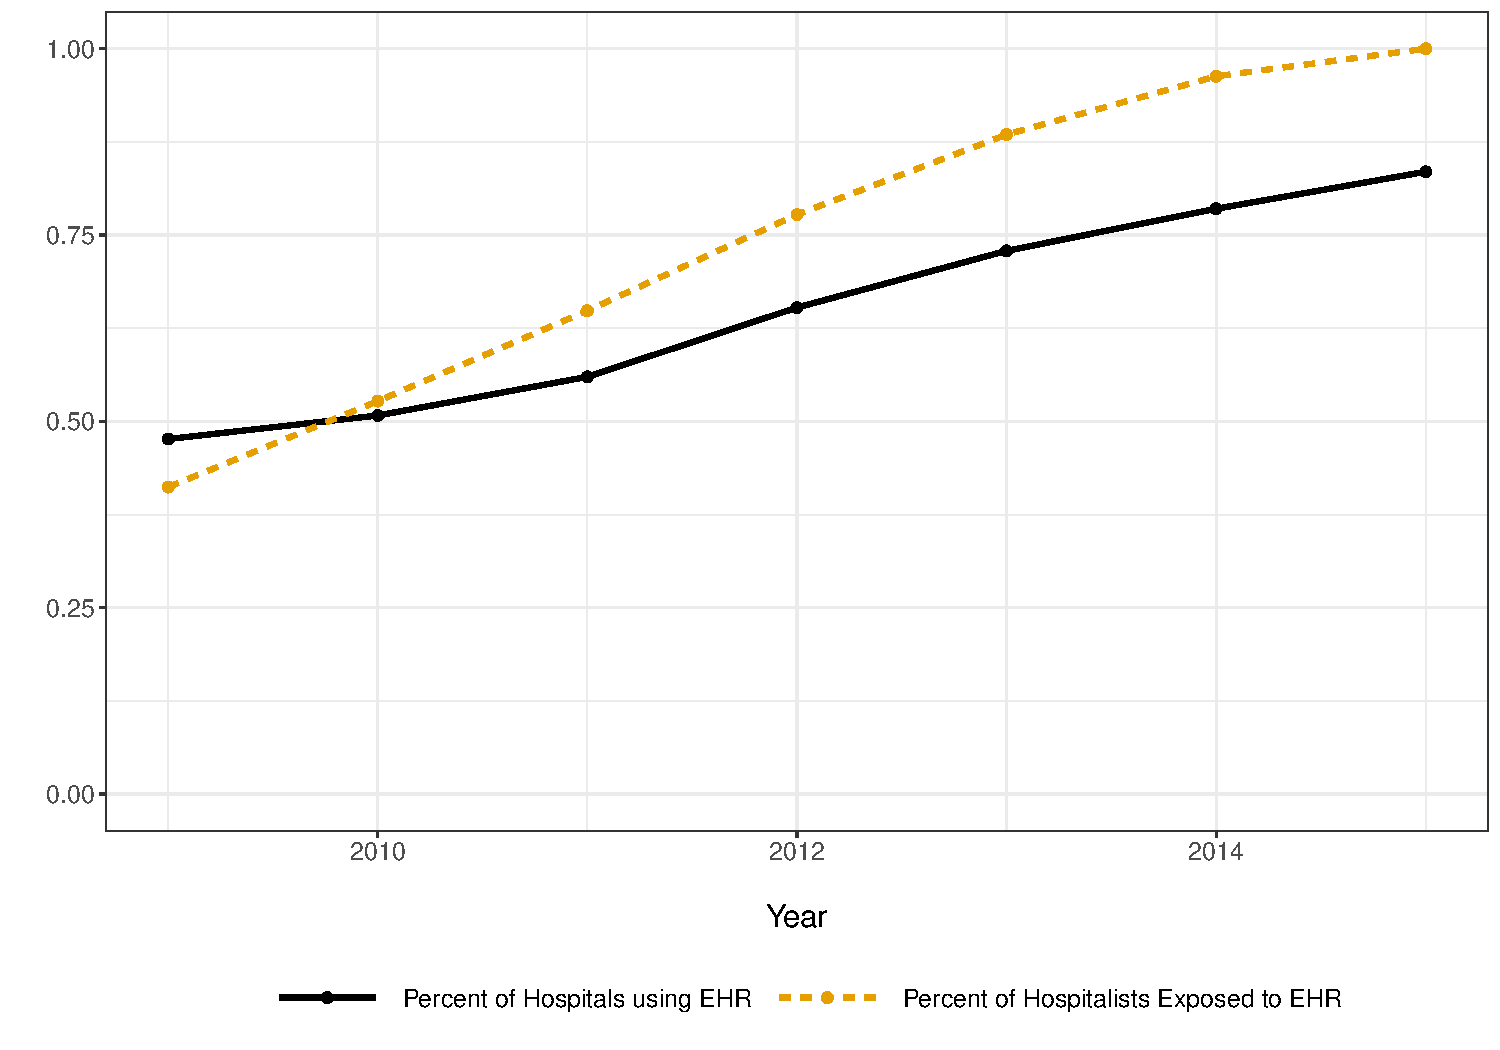
\includegraphics[scale=.5]{Objects/sum_stats_year.pdf}
\end{frame}


\section{Analysis}

\begin{frame}{Event Studies}


    
\end{frame}

\section{Results}

\begin{frame}{Dep. Variable: Patients Billed with Hospitals}
\begin{figure}[ht]
        \begin{minipage}[b]{0.47\linewidth}
            \centering
            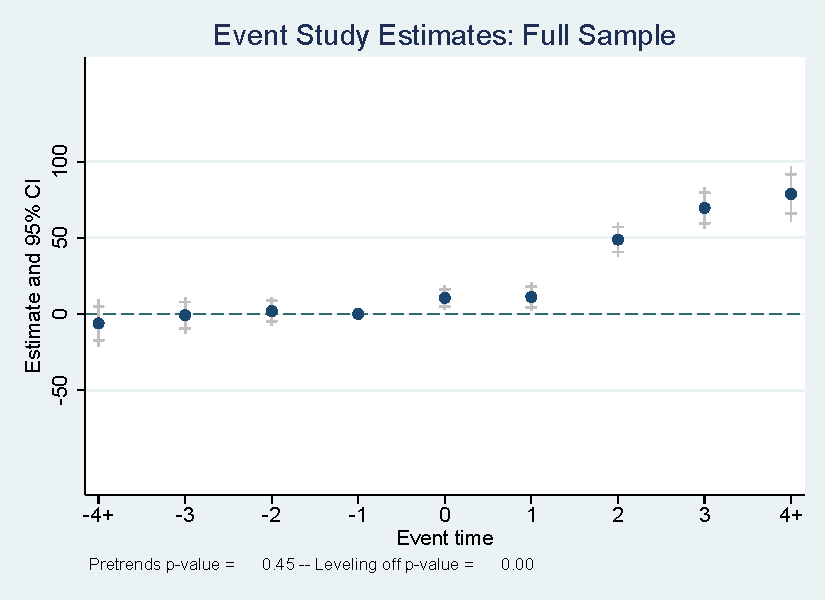
\includegraphics[width=\textwidth]{Objects/xtevent_fullsample.pdf}
            \caption{\small All Physicians\\}
        \end{minipage}
        \hspace{0.2cm}
        \begin{minipage}[b]{0.47\linewidth}
            \centering
            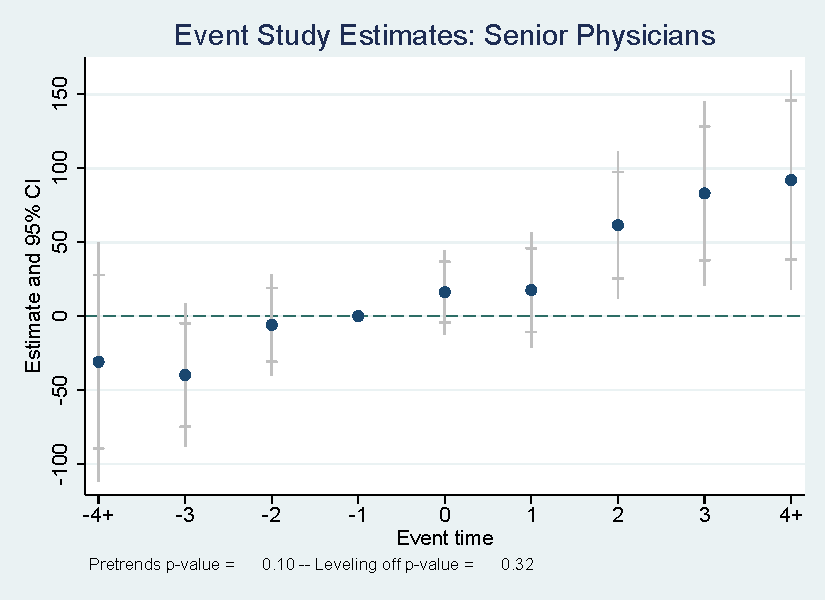
\includegraphics[width=\textwidth]{Objects/xtevent_oldsample.pdf}
            \caption{\small Phys. $>$ 35 yrs Experience}
        \end{minipage}
    \end{figure}
\end{frame}

\begin{frame}{Dep. Variable: Patients Billed with Hospitals}
\begin{figure}[ht]
        \begin{minipage}[b]{0.47\linewidth}
            \centering
            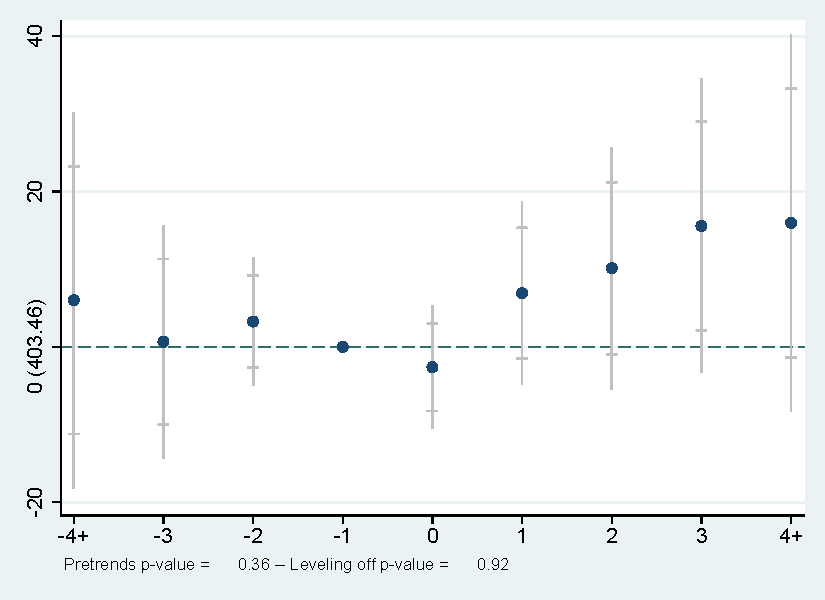
\includegraphics[width=\textwidth]{Objects/xtevent_hosp_fullsample.pdf}
            \caption{\small All Physicians \\(Only 1 Hospital)}
        \end{minipage}
        \hspace{0.2cm}
        \begin{minipage}[b]{0.47\linewidth}
            \centering
            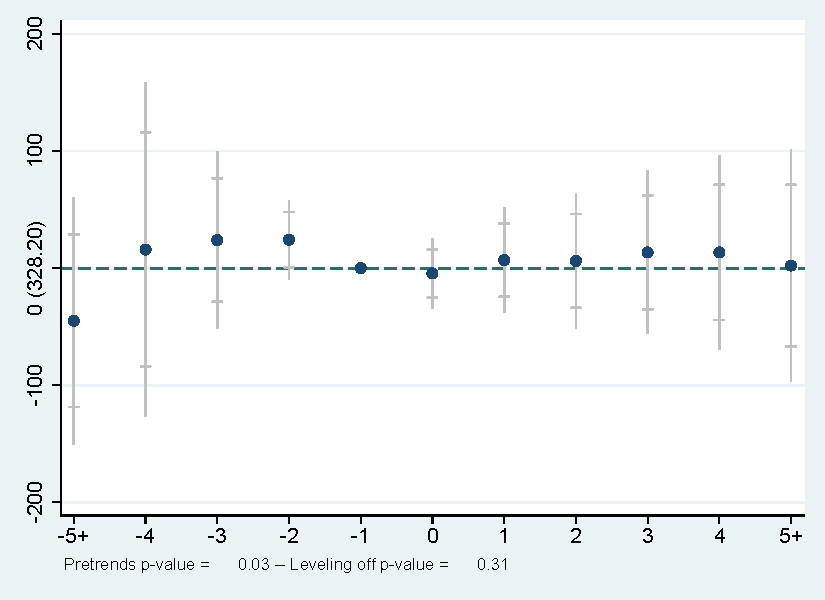
\includegraphics[width=\textwidth]{Objects/xtevent_hosp_oldsample.pdf}
            \caption{\small Phys. $>$ 35yrs\\ (Only 1 Hospital)}
        \end{minipage}
    \end{figure}
\end{frame}


\begin{frame}{Dep. Variable: Probability of Billing, but not With Hospitals}
\begin{figure}[ht]
        \begin{minipage}[b]{0.47\linewidth}
            \centering
            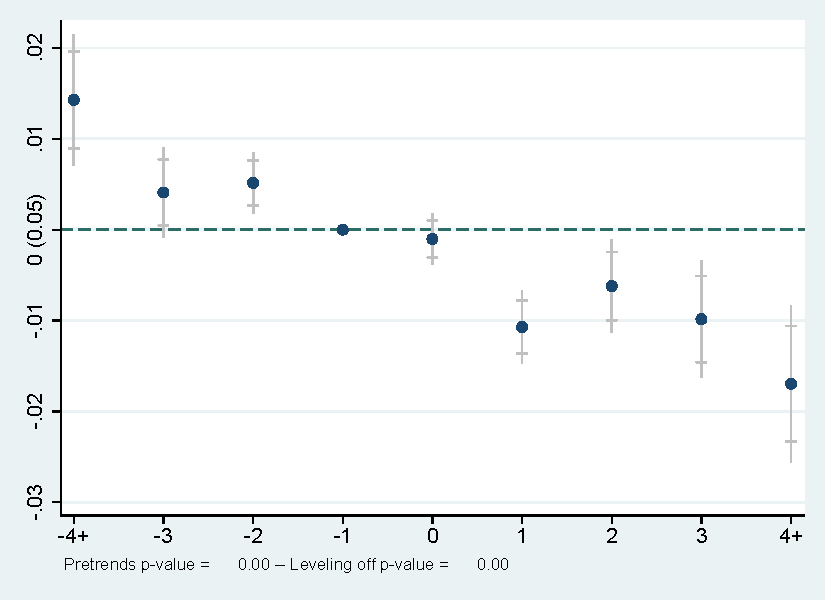
\includegraphics[width=\textwidth]{Objects/xtevent_fullsample_ind.pdf}
            \caption{\small All Physicians}
        \end{minipage}
        \hspace{0.2cm}
        \begin{minipage}[b]{0.47\linewidth}
            \centering
            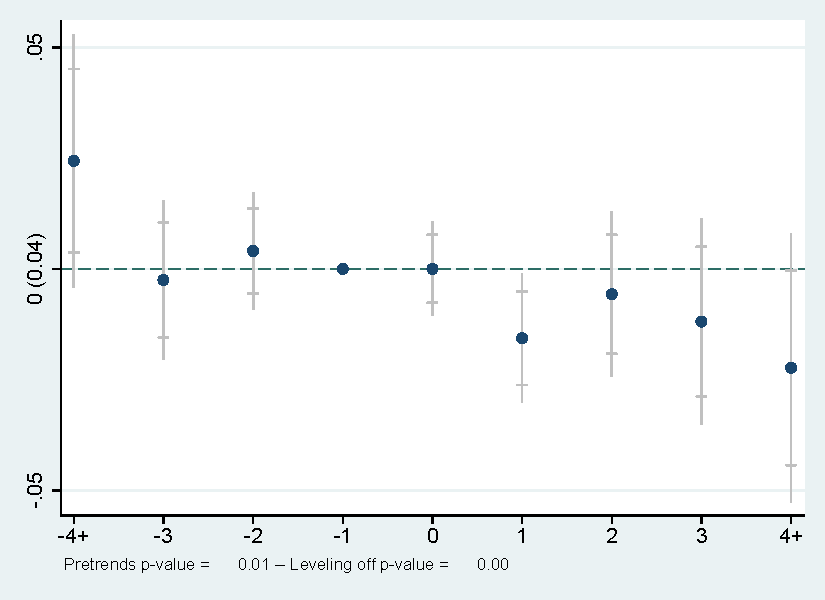
\includegraphics[width=\textwidth]{Objects/xtevent_oldsample_ind.pdf}
            \caption{\small Phys. $>$ 35yrs Experience}
        \end{minipage}
    \end{figure}
\end{frame}


\begin{frame}{Dep. Variable: Probability of Billing, but not With Hospitals}
\begin{figure}[ht]
        \begin{minipage}[b]{0.47\linewidth}
            \centering
            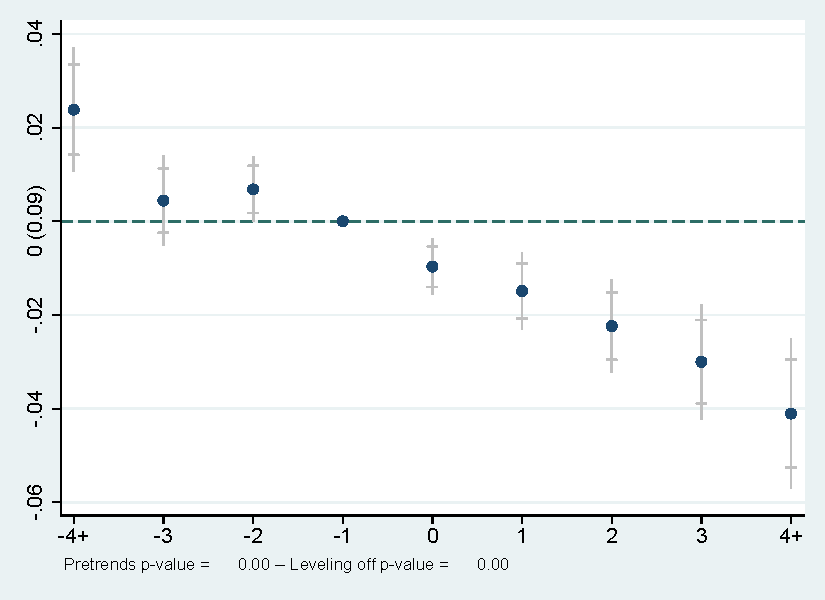
\includegraphics[width=\textwidth]{Objects/xtevent_hosp_fullsample_ind.pdf}
            \caption{\small All Physicians \\(Only 1 Hospital)}
        \end{minipage}
        \hspace{0.2cm}
        \begin{minipage}[b]{0.47\linewidth}
            \centering
            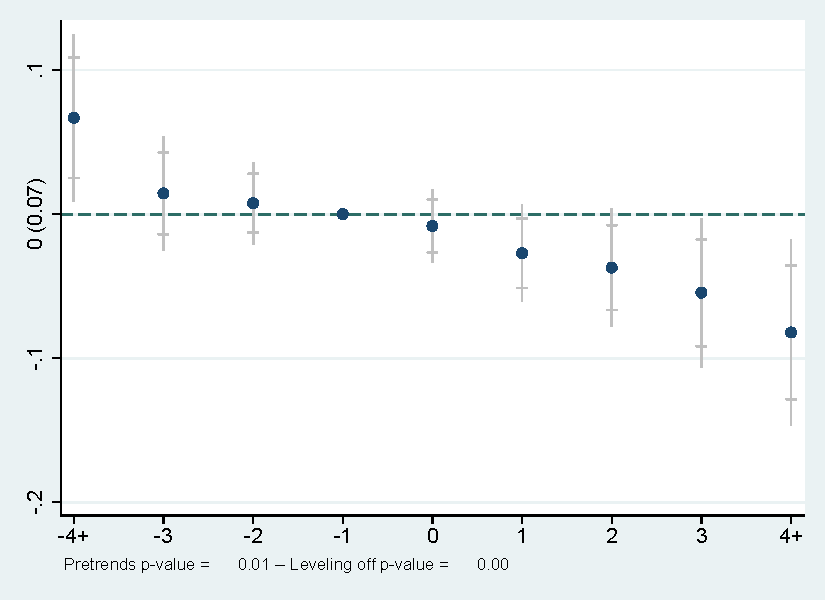
\includegraphics[width=\textwidth]{Objects/xtevent_hosp_oldsample_ind.pdf}
            \caption{\small Phys. $>$ 35yrs Experience\\ (Only 1 Hospital)}
        \end{minipage}
    \end{figure}
\end{frame}



\end{document}
